\documentclass{article}
\usepackage{graphicx}
\usepackage{algorithm}
\usepackage[noend]{algorithmic}
\usepackage{subfigure}
\usepackage{amssymb, amsmath, graphicx, charter, latexsym}
\usepackage{layouts}
\usepackage[letterpaper]{geometry}
\usepackage{enumerate}
\usepackage{epstopdf}
\usepackage{ragged2e}
%\usepackage{times}
\usepackage{mathtools}
%\usepackage[scaled]{helvet}
\usepackage{mathptmx}
\usepackage{verbatim}
\usepackage{listings}
\usepackage{siunitx}
\usepackage{booktabs}

\lstset{
basicstyle=\ttfamily,
}

\begin{document}

\title{\bf ECEN 689-- Real-Time Wireless Networks: Project 2\\ (Due on 4/1)}
\date{}
\author{%
Ping-Chun Hsieh\\
\texttt{lleyfede@tamu.edu}
\and
Tao Zhao\\
\texttt{alick@tamu.edu}
\and
Dongni Han\\
\texttt{handongni2015@tamu.edu}
}
\maketitle

\section*{Terminology}

In our report, we use ``server'' to denote the WiFi access point (AP), and
``client'' to denote the terminal device such as a mobile phone, a tablet, and
so on. Throughout our simulation, we let node $0$ be the server, and the other nodes be the clients. The basic time unit for packet transmission is called \emph{slot}, which should be greater than a round-trip time (RTT). For real-time traffic, we group an integer number (denoted by $T$) of slots into an \emph{interval}, which is the relative deadline of the packets. 

S-WiFi is the name of our application as well as our project. It stands for
Smart WiFi, or whatever you think it is.

\section*{Simulation Setup}
\begin{table}[htbp]
\centering
    \caption{Parameters of the wireless channel.}
    \vspace{2mm}
    \begin{tabular}{ | l | l | }
    \hline
    Item & Value \\ \hline
    Path loss exponent & 2.0  \\ \hline
    Shadowing deviation & \SI{4.0}{dB} \\ \hline
    Reference distance & \SI{1.0}{m} \\
    \hline
\end{tabular}
\label{table: channel}
\end{table}
Throughout the report, we consider a wireless network of one AP and $N$ clients, where $N>1$. The transmitter power level is \SI{1}{W}. We use the shadowing module as the wireless channel. The parameters of the channel are summarized in Table \ref{table: channel}. The channel reliability can be changed by varying the distance between the AP and the clients. In our simulation, we set the distance between the AP and a client to be $\SI{1}{m}$ when creating a reliable channel. For an unreliable channel with $p_n\approx 0.57$, the corresponding distance is $\SI{1000}{m}$. 

\begin{table}[htbp]
\centering
\caption{Parameters of the 802.11b MAC.}
    \vspace{2mm}
    \begin{tabular}{ | l | l | }
    \hline
    Item & Value \\ \hline
    Data rate & \SI{11}{Mb/s}  \\ \hline
    Basic rate & \SI{1}{Mb/s}  \\ \hline
    PLCP data rate & \SI{1}{Mb/s}  \\ \hline 
    Preamble length & \SI{144}{bits} \\ \hline
    Slot time & \SI{20}{\mu s} \\ \hline
    SIFS & \SI{10}{\mu s} \\
    \hline
\end{tabular}
\label{table: mac}
\end{table}

For the medium access control (MAC) layer, we use the 802.11 module built in ns-2. Following the IEEE 802.11b standard, the MAC layer parameters are chosen as in Table \ref{table: mac}. In this project, the automatic retry function built in 802.11 is disabled, i.e. \lstinline|ShortRetryLimit_| and \lstinline|LongRetryLimit_| are set to be 0 in the Tcl domain, to avoid channel congestion due to uncontrollable retransmission in the MAC layer.

Since ns-2 has no PCF module, we mimic PCF in the application layer. Throughout the simulation, a slot is chosen to be $\SI{10}{ms}$, which is much longer than a RTT ($\approx\SI{1.63}{ms}$), to guarantee enough margin for packet delivery.


\section*{Uplink Transmissions with PCF}
\label{section: uplink}
For the centralized networks described above, we consider uplink transmission with  PCF from the clients to the AP. In PCF mode, the AP has full control over channel allocation. In the beginning of each interval, each client generates a random number of packets and waits for channel access that is fully controlled by the AP. Since the packets are generated and queued on the client's side, the AP needs to collect the queue information of the clients to make scheduling decisions. The baseline policy is described in Section \ref{section: baseline}.


\section{Baseline Policy}
\label{section: baseline}


\frenchspacing  Under the baseline policy, there are two phases in each interval. In the \emph{polling phase}, the AP collects the queue information by polling each client in a round-robin fashion. In the \emph{scheduling phase}, the AP schedules one of the clients based on the queue information and channel reliability.

\subsection{Polling Phase}
In the beginning of each interval, the AP gathers the queue information by sending \lstinline|SWiFi_POLL_NUM| packets to each client based on round-robin policy. Upon receiving the \lstinline|SWiFi_POLL_NUM|, the client will reply with a \lstinline|SWiFi_PKT_NUM_UL| packet which contains the queue information in the packet header. If either the transmission of \lstinline|SWiFi_POLL_NUM| or \lstinline|SWiFi_PKT_NUM_UL| fails, the AP will retransmit the \lstinline|SWiFi_POLL_NUM| packet again to the same client in the next slot. 
The polling phase ends when the AP receives all the queue information from the clients.

In the real-time scenario, the queue information is referred to as the number of packets generated in the current interval. On the other hand, for the non-real-time traffic, the queue information corresponds to the total number of packets received up to the present (denoted by $X_n$), which is used by the AP to obtain the real queue length of each client.    
%The AP will first send a POLL packet to the selected client. A client can only transmit its packet after it receives the POLL packet from the AP. This allows the AP to have full control over which client transmits. 

%Baseline policy: At the beginning of each interval, the AP asks each client, one by one, the number of packets that it generates. After this process, the AP also knows the number of packets at each client, and it can make the best decision.
\subsection{Scheduling Phase}
In each slot of the scheduling phase, the AP applies the Max-Weight policy, which schedules the client that maximizes the product of the queue length and the channel reliability. The AP sends a \lstinline|SWiFi_PKT_POLL_DATA| packet to the target client to provide access to the channel. When the scheduled client receives the data polling request, it will reply a packet of type \lstinline|SWiFi_PKT_DATA_UL| immediately to the AP. If the AP receives the data packet successfully, the AP will decrease the queue length by 1. If either the transmission of data polling or the data packet fails, the AP will stay with the same schedule in the next slot (suppose the next slot is not the end of the interval). Note that in the non-real-time scenario, in order to derive the real queue length of each client, the AP needs to keep track of the total number of received packets (denoted by $Y_n$) from each client $n$, and then calculates the queue length as $(X_n - Y_n)$ for each client $n$.

If the AP already receives all the packets available in the current interval, it will simply idle until the start of the next interval.

%Besides, we define four data types. 
     

\section{Implementation in NS-2}
\label{section: ns2}
\begin{table}[htbp]
   \centering
   \caption{Data Type}
   \label{tab:table3}
   \begin{tabular}{| l | l |}
      \hline
      Data Type  &  Meaning\\ \hline
      \lstinline|SWiFi_POLL_NUM| & Poll number of packets in uplink\\ \hline 
      \lstinline|SWiFi_PKT_POLL_DATA|  & Poll data packet transmission in uplink\\ \hline 
      \lstinline|SWiFi_PKT_NUM_UL| & Packet in uplink that carries number of packets at client\\ \hline 
      \lstinline|SWiFi_PKT_DATA_UL| & Data packet in uplink(client to server)\\  
     \hline
   \end{tabular}
\end{table}
 
What's more, four poll states are defined below. 
\begin{table}[htbp]
   \centering
   \caption{Poll State}
   \label{tab:table4}
   \begin{tabular}{| l | l |}
      \hline
      Poll State  &  Meaning\\ \hline
      \lstinline|SWiFi_POLL_NONE| & Poll nothing\\ \hline 
      \lstinline|SWiFi_POLL_NUM|  & Poll num of packets\\ \hline 
      \lstinline|SWiFi_POLL_DATA| & Poll data\\ \hline 
      \lstinline|SWiFi_POLL_IDLE| & Idle\\  
     \hline
   \end{tabular}
\end{table}
In our SWiFi project, the way we implement baseline policy is described as follows. 

In the \lstinline|command| function in swifi.cc

When the system captures a string called  \lstinline|server| indicating that it is a server(AP). If the value of  \lstinline|do_pull_num|  is true,  \lstinline|poll_state_|  will be set to  \lstinline|SWiFi_POLL_NUM|. Otherwise, when the value of  \lstinline|do_pull_num|  is false,   \lstinline|poll_state_|  will be set  \lstinline|SWiFi_POLL_DATA|. 


When the system captures a string called  \lstinline|poll|, tcl will print an error: only server AP can poll if it's not a server. If it's a server, the server(AP) will ask each client one by one using function \lstinline|scheduleRoundRobin| when the \lstinline|poll_state_| is  \lstinline|SWiFi_POLL_NUM|. And we set the packet type to \lstinline|SWiFi_PKT_POLL_NUM|, store current time and send the new packet. Otherwise, the server(AP) will use maxweight policy to schedule clients using function \lstinline|scheduleMaxWeight| when the \lstinline|poll_state_| is  \lstinline|SWiFi_POLL_DATA|. And we set the packet type to \lstinline|SWiFi_PKT_POLL_DATA|, store current time and send the new packet. Besides, there is one special condition that no more client is left in one interval (\lstinline|target_| is true). In this case, \lstinline|poll_state_| will be set to \lstinline|SWiFi_POLL_IDLE|.


When the system captures a string \lstinline|boi|, the system will set \lstinline|target_| to NULL. If  \lstinline|realtime_|  is true indicating it is real-time traffic, we need clear number of data packets of all clients at the beginning of each interval. 

In the  \lstinline|recv| function in swifi.cc

When a client receives a packet type \lstinline|SWiFi_PKT_POLL_DATA| transmitted by a server, we save the old packet's send time, discard the old packet, create a new packet, set new send time and send this new packet to the server(AP). 
When a client receives a packet type \lstinline|SWiFi_PKT_POLL_NUM| transmitted by a server, we set the data type to \lstinline|SWiFi_PKT_NUM_UL| meaning that it is uplink packet with numbers of packets at client, set new send time and send this new packet to the server(AP).
When a server receivers  a packet type \lstinline|SWiFi_PKT_NUM_UL| transmitted by a client, the current queue length is equal to the number of data packets generated minus the number of data packets received. For real-time traffic, the current queue length is equal to the number of data packets generated.  

For Real-time traffic: At the beginning of each interval, we need clean queues of all clients cause we don't need store the queue length last interval. The current queue length just equals random number of packets at the beginning of each interval. 

For Non-real-time traffic: We need store the queue length last interval. The current queue length is equal to the number of data packets generated minus the number of data packets received. 

\section{Simulation Results}
\label{section: simulation}
\subsection{Symmetric System with 2 Clients}
Under the simulation setup described above, the real-time 
Real-time and non-real-time traffic
\subsection{Asymmetric System with 2 Clients}

\subsection{System with N Clients}
%\begin{figure}[htbp]
%\centering
%\subfigure[Downlink round-trip time.]{
%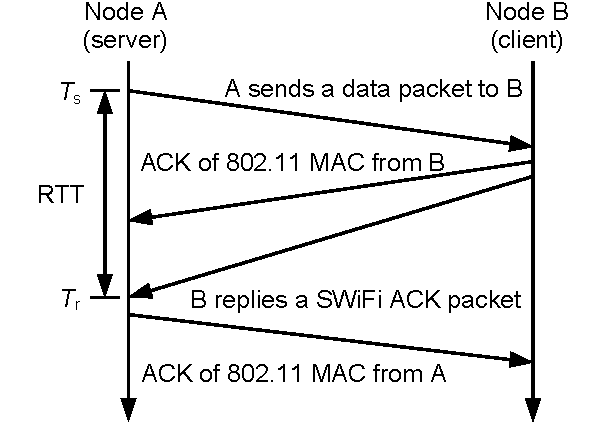
\includegraphics[scale = 0.7]{downlink_rtt.pdf}}
%\subfigure[Uplink round-trip time.]{
%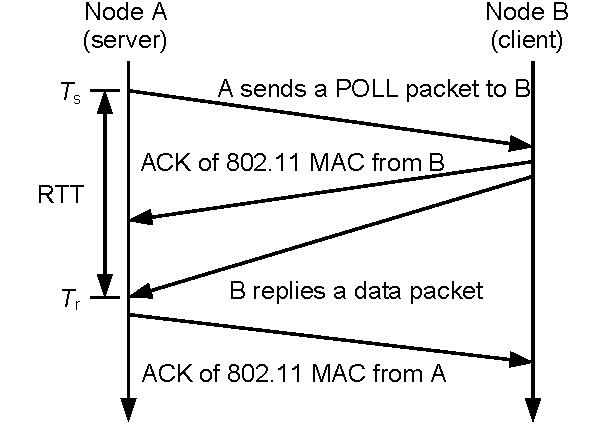
\includegraphics[scale = 0.7]{uplink_rtt.pdf}}
%\caption{Round-trip time when node A and node B are close to each other.}
%\label{figure: rtt}
%\end{figure}


\end{document}
